% Generated from tex/chapters/ch04/08_構築技術.tex for the SWEBOK structure tree
\subsubsection{API の設計と利用}

API は、ライブラリやフレームワーク、サービスを利用するために公開された操作の集合である。API は、関数名や引数の型といった署名だけでなく、その操作が何を意味し、どのような効果を持つかという意味も含む。

よい API は、学びやすく、覚えやすく、読みやすいコードにつながり、誤用しにくく、拡張しやすく、必要な機能を十分に備え、後方互換性を保ちやすい。広く使われるライブラリやサービスでは、実装よりも API の方が長く生きることが多いため、API は安定性が重要である。

Web API では、RESTful API や OpenAPI のような標準的な記述がよく使われる。API ファーストとは、アプリケーションの内部実装より先に API の契約を設計し、その契約に基づいてサーバ側とクライアント側を作る考え方である。

\begin{figure}[htbp]
\centering
\IfFileExists{assets/fig-ch04-08.png}{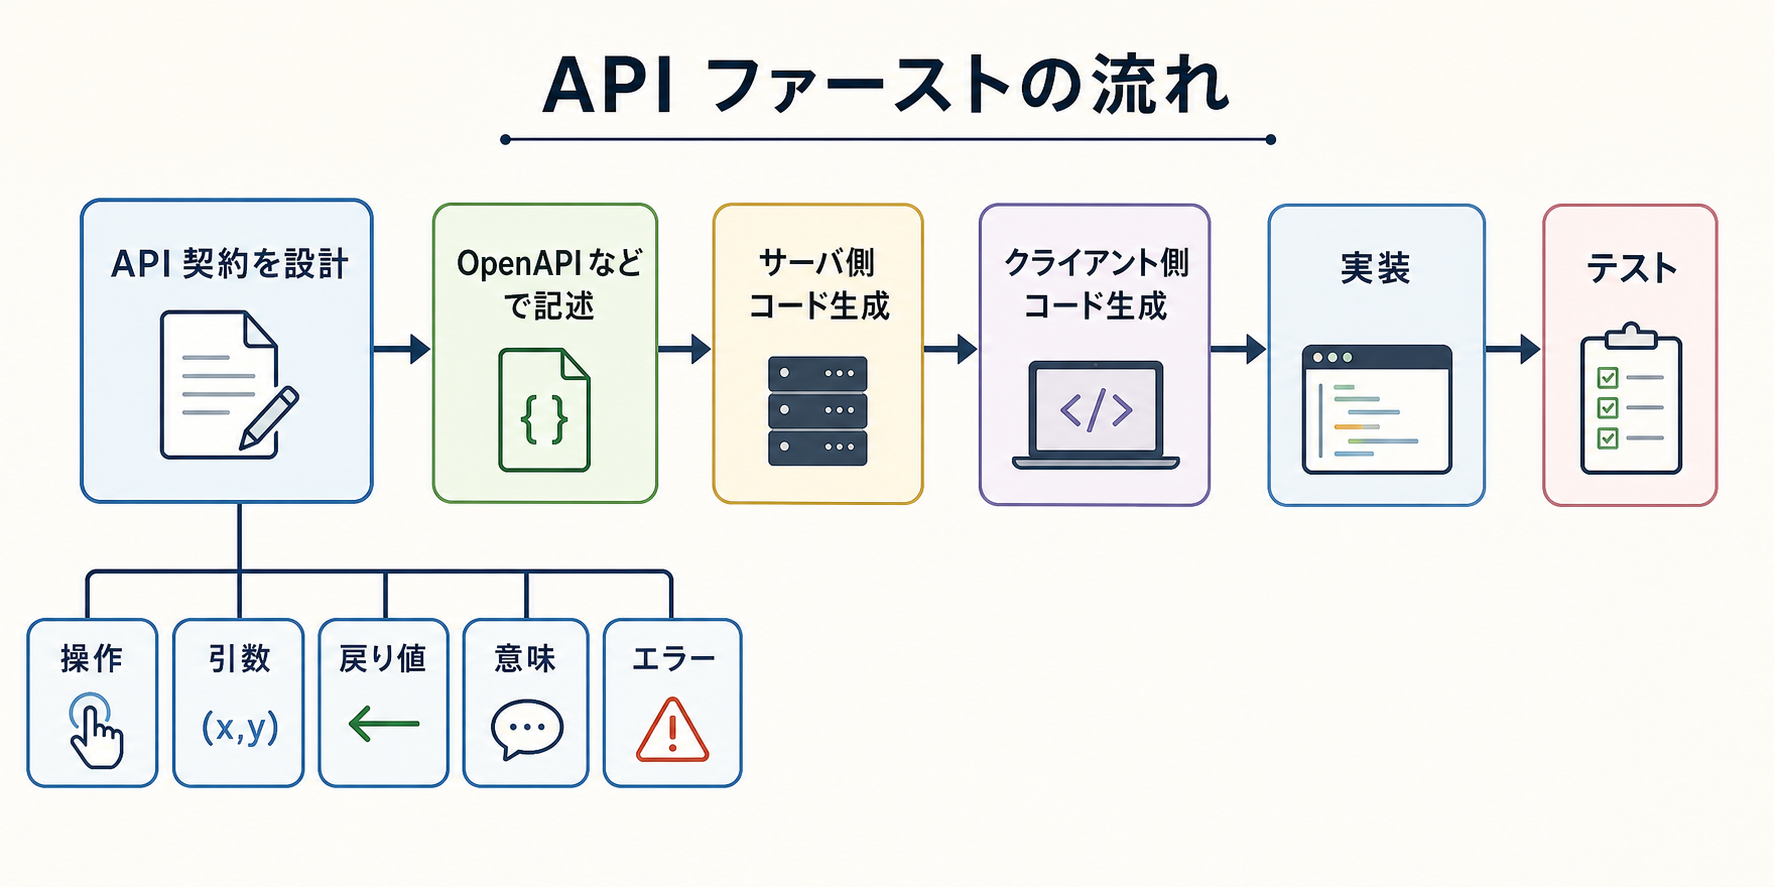
\includegraphics[width=0.96\linewidth]{assets/fig-ch04-08.png}}{\fbox{\parbox[c][48mm][c]{0.9\linewidth}{\centering 画像生成待ち\\API ファーストの流れ}}}
\caption{API ファーストの流れ}
\label{fig:ch04-08}
\end{figure}
